\section{Messung der Lebensdauer kosmischer Myonen}
\label{sec:messung}
In diesem Abschnitt wird die Bestimmung der Lebensdauer kosmischer Myonen
vorgestellt.
Zunächst muss hierfür die Messapparatur kalibriert werden.
Außerdem wird durch Messung der Myonen-Zählrate unter Variation der
Verzögerungsleitungen eine Zeitauflösung der Apparatur ermittelt.
Alle Fehler werden im Folgenden mit Hilfe des \texttt{python}-
Paketes \texttt{uncertainties} berechnet, das eine automatische
Gauß\'sche Fehlerfortpflanzung anbietet.

\subsection{Zeitkalibration der Apparatur}
\label{subsec:kalibration}
Die auszuwertenden Daten werden in dieser Messung mit Hilfe eines
Vielkanalanalysators (VKA) gewonnen.
Dieser liefert Histogramm-Daten von Myonen-Kandidaten, die in \num{512} Kanäle
eingeteilt sind.
Die Kanalnummer $C_i$ eines Ereignisses hängt dabei linear mit der
Zeit $t_i$ des entsprechenden Myon-Kandidaten zwischen Start- und
Stopp-Impuls zusammen:
\begin{equation}
    t_i = a + b \cdot C_i\,,
\end{equation}
mit den Koeffizienten $a$ und $b$, die im Folgenden bestimmt werden.

Zur Kalibration der Apparatur werden in zeitlich konstanten Abständen
Signalimpulse auf den VKA gegeben.
Diese Impulse füllen jeweils einen spezifischen Kanal, wobei die Entsprechende
Zeit $t_i$ bekannt ist.
Durch Einstellung verschiedener Signalzeiten können mehreren Kanälen eine
Zeit zugeordnet werden.
Die Software \texttt{Maestro V6.06} des VKA führt daraufhin eine lineare Ausgleichsrechnung mit diesen
Kanälen durch und liefert so die Parameter
\begin{align*}
     a &= \SI{0.023}{\micro \second}\\
     \text{und} \quad b &= \SI[per-mode=fraction]{0.047}{\micro \second \per {Kanal}} \,.
 \end{align*}
 Im Folgenden wird lediglich der Parameter $b$ von Interesse sein.

\subsection{Zeitauflösung der Apparatur}
\label{subsec:zeitaufloesung}
Um verschiedene Signallaufzeiten der beiden SEV auszugleichen, werden vor der
Messung Verzögerungsleitungen angeschlossen, die eine zusätzliche
Verzögerungszeit $T_\text{VZ}$ einbringen.
Durch Messung der Myonen-Zählraten unter Variation der Verzögerungszeit
lässt sich so eine Auflösungszeit $\Delta t_\text{K}$ der Koinzidenzeinheit
als Breite einer Gaußkurve bestimmen.
Die Messwerte sind in Tabelle \ref{tab:resolution} aufgeführt, Abbildung
\ref{fig:resolution} zeigt den Fit einer Gauß-Funktion an die Datenpunkte,
welcher die folgende Auflösungszeit liefert:
\begin{equation*}
    \Delta t_\text{K} = \SI{4.50+-0.11}{\nano \second}\,.
\end{equation*}
Die weiteren Messungen werden bei maximaler Zählrate durchgeführt, was bei
einer Verzögerungszeit $T_\text{VZ} = \SI{0.5}{\nano \second}$ erreicht wird.
\begin{figure}[htb]
    \centering
    \includegraphics[width=0.7\linewidth]{img/resolution.pdf}
    \caption{
        Myonenrate in Abhängigkeit der effektiven Signalverzögerung
        $T_\text{VZ}$.
    }
    \label{fig:resolution}
\end{figure}
\begin{table}
    \centering
    \caption{
        Messwerte zur Bestimmung der zu verwendenden Verzögerungsleitung
        und Auflösungszeit $\Delta t_\text{K}$ der Koinzidenzeinheit.
    }
    \label{tab:resolution}
    \begin{tabular}{SSSSS}
        \toprule
        {Leitung 1} & {Leitung 2} & {$T_\text{VZ}$} & {Ereignisse} & {Rate [\si{\hertz}]} \\
        \midrule
        16.0 & 0.0  &  -16.0 &     0 &    0.00 \\
        16.0 & 2.0  &  -14.0 &     1 &    0.03 \\
        16.0 & 4.0  &  -12.0 &     1 &    0.03 \\
        16.0 & 6.0  &  -10.0 &    14 &    0.47 \\
        16.0 & 8.0  &   -8.0 &    63 &    2.10 \\
        16.0 & 10.0 &   -6.0 &   179 &    5.97 \\
        16.0 & 12.0 &   -4.0 &   261 &    8.70 \\
        16.0 & 14.0 &   -2.0 &   408 &   13.60 \\
        16.0 & 14.5 &   -1.5 &   389 &   12.97 \\
        16.0 & 15.0 &   -1.0 &   385 &   12.83 \\
        16.0 & 15.5 &   -0.5 &   409 &   13.63 \\
        16.0 & 16.0 &    0.0 &   436 &   14.53 \\
        16.0 & 16.5 &    0.5 &   444 &   14.80 \\
        16.0 & 17.0 &    1.0 &   392 &   13.07 \\
        16.0 & 18.0 &    2.0 &   417 &   13.90 \\
        16.0 & 20.0 &    4.0 &   324 &   10.80 \\
        16.0 & 22.0 &    6.0 &   191 &    6.37 \\
        16.0 & 24.0 &    8.0 &   104 &    3.47 \\
        16.0 & 26.0 &   10.0 &    34 &    1.13 \\
        16.0 & 28.0 &   12.0 &     8 &    0.27 \\
        16.0 & 30.0 &   14.0 &     4 &    0.13 \\
        16.0 & 32.0 &   16.0 &     3 &    0.10 \\
        \bottomrule
    \end{tabular}
\end{table}

\clearpage
\subsection{Untergrundrate}
\label{subsec:untergrund}
Zur Abschätzung der Anzahl $N_\text{Bkg}$ der Untergrundereignisse wird
die Wahrscheinlichkeit betrachtet,
mit der ein Myon in einem zuvor gestarteten Messintervall der Länge
$T_\text{S} = \SI{10}{\micro \second}$ ein Stopp-Signal erzeugt.
Unter der Annahme, dass die Myonen normalverteilt auftreten,
lässt sich die Wahrscheinlichkeit $p_i$ einer Messung von $i$ Myonen im
gegebenen Zeitintervall durch die Poissonverteilung abschätzen:
\begin{equation*}
    p_i = \frac{\lambda^i}{i!}\mathrm{e}^{-\lambda}\,.
\end{equation*}
Der Erwartungswert der Messung eines Myons wird dabei mit $\lambda$
bezeichnet und entspricht $\lambda = T_\text{S}f$, wobei $f$ die Zählrate ist.
Hier wird die maximale Zählrate von $f = \SI{14.8}{\hertz}$ angesetzt,
welche schließlich eine Wahrscheinlichkeit der Messung eines Myons von
\begin{equation*}
    p = \lambda \mathrm{e}^{-\lambda} = \SI{0.0149(9)}{\percent}
\end{equation*}
ergibt.
Bei einer Messdauer von etwa $T_\text{M} = \SI{88}{h}$ sind damit
\begin{equation*}
    N_\text{Bkg} = T_\text{M}fp = \num{47.0+-2.7}
\end{equation*}
Untergrundereignisse zu erwarten.

\subsection{Lebensdauerbestimmung}
\label{subsec:lebensdauer}
Abschließend wird die Lebensdauer der Myonen bestimmt.
Hierzu wird mit einem Fit einer Funktion der Form \eqref{eqn:exponential}
and die Daten des VKA der Parameter $\gamma$ bestimmt.
Zur Berücksichtigung der Untergrundrate werden pro Kanal \num{0.1} Ereignisse
abgezogen, was besonders im Bereich kleiner Myonen-Zerfallszeiten einen
vernachlässigbaren Anteil ausmacht.

Zur Berechnung der kalibrierten Lebensdauer $\tau$ wird der Kehrwert des
Parameters $\gamma$ gebildet und mit dem zuvor bestimmten Wert $b$ der
Kalibrationsfunktion multipliziert:
\begin{equation*}
    \tau = \frac{1}{\gamma} b \,.
\end{equation*}
Der in Abbildung \ref{fig:fit} dargestellte Fit liefert schließlich
\begin{align*}
    \gamma &= \SI{0.02125+-0.00021}{\per {Kanal}}\\
    \Rightarrow \quad \tau_\mu &= \SI{2.19+-0.05}{\micro \second}\..
\end{align*}
\begin{figure}[htb]
    \centering
    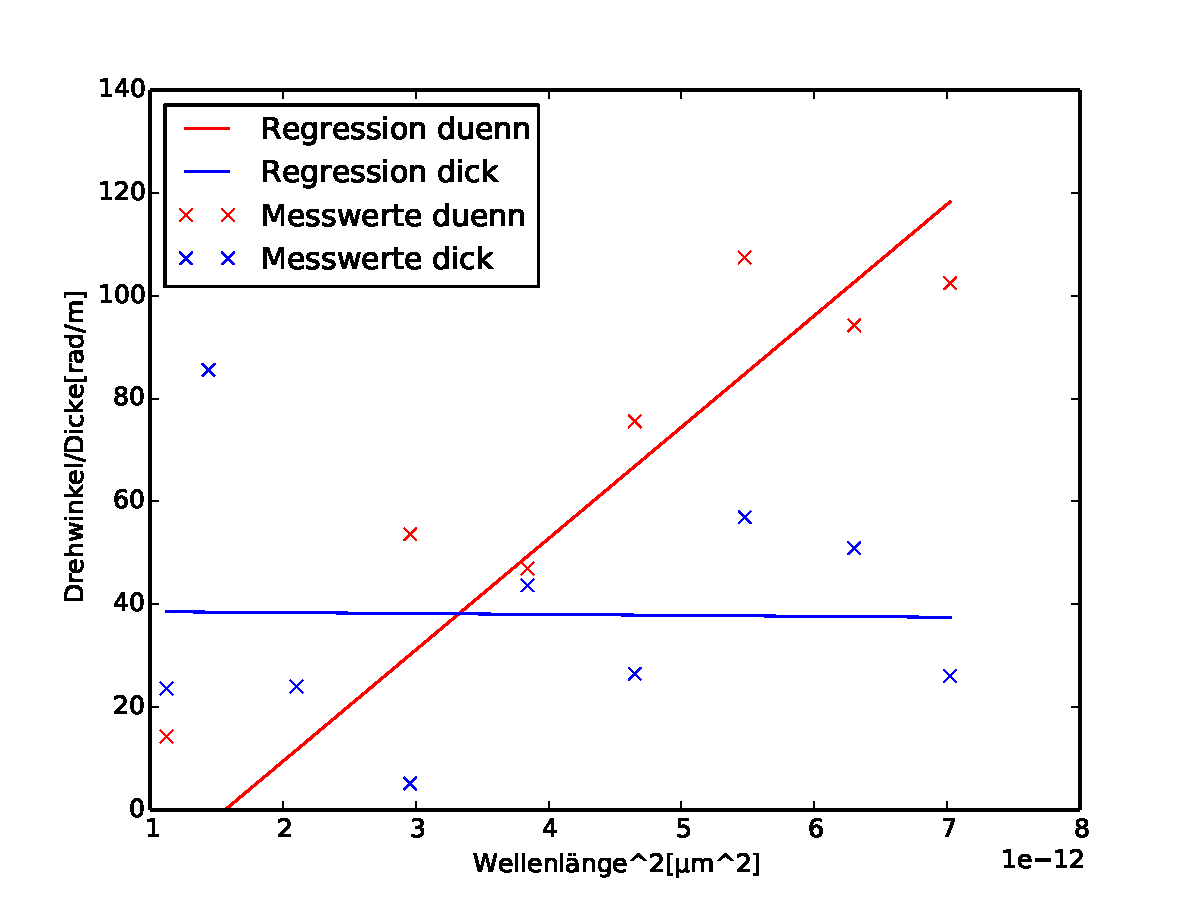
\includegraphics[width=0.7\linewidth]{img/fit.pdf}
    \caption{
        Bestimmung der Zerfallskonstante der Myonen. Durch Fit einer
        Exponentialfunktion an die Datenpunkte wird diese bestimmt.
        Mit Kenntnis einer Kalibrationsfunktion kann somit die Lebensdauer
        der kosmischen Myonen berechnet werden.
        Die Statistischen Unsicherheiten sind zur besseren Übersichtlichkeit
        nicht aufgeführt.
    }
    \label{fig:fit}
\end{figure}

\section{Diskussion}
\label{sec:diskussion}
Das Ergebnis dieser Messung stimmt innerhalb der Fehler mit den bekannten
Werten der Myonen-Lebensdauer von $\tau_{\mu,\text{lit}} = \SI{2.1969811+-0.0000022}{\micro \second}$ \cite{pdgonline} überein.
Die Unsicherheiten der Messung sind mit etwa \SI{2}{\percent}
ausgesprochen klein.
Im Nachhinein wäre eine nachträgliche Zeitkalibration der Apparatur
einer direkten Kalibration vorzuziehen, um diesen Schritt insgesamt
transparenter zu gestalten.
